\documentclass{beamer}
\usepackage{amsmath}
\usepackage[english]{babel} %set language; note: after changing this, you need to delete all auxiliary files to recompile
\usepackage[utf8]{inputenc} %define file encoding; latin1 is the other often used option
\usepackage{csquotes} % provides context sensitive quotation facilities
\usepackage{graphicx} %allows for inserting figures
\usepackage{booktabs} % for table formatting without vertical lines
\usepackage{textcomp} % allow for example using the Euro sign with \texteuro
\usepackage{stackengine}
\usepackage{wasysym}
\usepackage{tikzsymbols}
\usepackage{textcomp}
\newcommand{\bubblethis}[2]{
        \tikz[remember picture,baseline]{\node[anchor=base,inner sep=0,outer sep=0]%
        (#1) {\underline{#1}};\node[overlay,cloud callout,callout relative pointer={(0.2cm,-0.7cm)},%
        aspect=2.5,fill=yellow!90] at ($(#1.north)+(-0.5cm,1.6cm)$) {#2};}%
    }%
\tikzset{face/.style={shape=circle,minimum size=4ex,shading=radial,outer sep=0pt,
        inner color=white!50!yellow,outer color= yellow!70!orange}}
%% Some commands to make the code easier
\newcommand{\emoticon}[1][]{%
  \node[face,#1] (emoticon) {};
  %% The eyes are fixed.
  \draw[fill=white] (-1ex,0ex) ..controls (-0.5ex,0.2ex)and(0.5ex,0.2ex)..
        (1ex,0.0ex) ..controls ( 1.5ex,1.5ex)and( 0.2ex,1.7ex)..
        (0ex,0.4ex) ..controls (-0.2ex,1.7ex)and(-1.5ex,1.5ex)..
        (-1ex,0ex)--cycle;}
\newcommand{\pupils}{
  %% standard pupils
  \fill[shift={(0.5ex,0.5ex)},rotate=80] 
       (0,0) ellipse (0.3ex and 0.15ex);
  \fill[shift={(-0.5ex,0.5ex)},rotate=100] 
       (0,0) ellipse (0.3ex and 0.15ex);}

\newcommand{\emoticonname}[1]{
  \node[below=1ex of emoticon,font=\footnotesize,
        minimum width=4cm]{#1};}
\usepackage{scalerel}
\usetikzlibrary{positioning}
\usepackage{xcolor,amssymb}
\newcommand\dangersignb[1][2ex]{%
  \scaleto{\stackengine{0.3pt}{\scalebox{1.1}[.9]{%
  \color{red}$\blacktriangle$}}{\tiny\bfseries !}{O}{c}{F}{F}{L}}{#1}%
}
\newcommand\dangersignw[1][2ex]{%
  \scaleto{\stackengine{0.3pt}{\scalebox{1.1}[.9]{%
  \color{red}$\blacktriangle$}}{\color{white}\tiny\bfseries !}{O}{c}{F}{F}{L}}{#1}%
}
\usepackage{fontawesome} % Social Icons
\usepackage{epstopdf} % allow embedding eps-figures
\usepackage{tikz} % allows drawing figures
\usepackage{amsmath,amssymb,amsthm} %advanced math facilities
\usepackage{lmodern} %uses font that support italic and bold at the same time
\usepackage{hyperref}
\usepackage{tikz}
\usepackage{tcolorbox}

\usefonttheme[onlymath]{serif} %set math font to serif ones

\definecolor{beamerblue}{rgb}{0.2,0.2,0.7} %define beamerblue color for later use

%%% defines highlight command to set text blue
\newcommand{\highlight}[1]{{\color{blue}{#1}}}


%%%%%%% commands defining backup slides so that frame numbering is correct

\newcommand{\backupbegin}{
   \newcounter{framenumberappendix}
   \setcounter{framenumberappendix}{\value{framenumber}}
}
\newcommand{\backupend}{
   \addtocounter{framenumberappendix}{-\value{framenumber}}
   \addtocounter{framenumber}{\value{framenumberappendix}}
}

%%%% end of defining backup slides

%Specify figure caption, see also http://tex.stackexchange.com/questions/155738/caption-package-not-working-with-beamer
\setbeamertemplate{caption}{\insertcaption} %redefines caption to remove label "Figure".
%\setbeamerfont{caption}{size=\scriptsize,shape=\itshape,series=\bfseries} %sets figure  caption bold and italic and makes it smaller

\newtcolorbox{boxA}{
    fontupper = \bf,
    boxrule = 1.5pt,
    colframe = black % frame color
}

\usetheme{Boadilla}

% --------------------
% Overall information
% --------------------
\title[Economía I]{Economía I \vspace{4mm}
\\ Magistral 20: Teoría de crecimiento}
\date{}
\author[Riottini]{Riottini Franco}
\vspace{0.4cm}
\institute[]{Universidad de San Andrés} 


\begin{document}

\begin{frame}
\titlepage
\centering


\includegraphics[scale=0.2]{../Figures/logoUDESA.jpg} 
\end{frame}

\begin{frame}
\frametitle{Tomemos una economía}
\begin{center}
    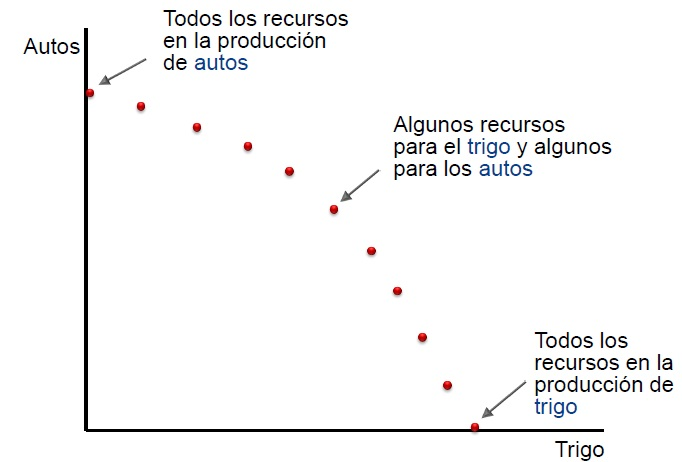
\includegraphics[scale=0.6]{../Tema_11.2_tomemosunaeconomia.jpg}
\end{center}
\end{frame}

\begin{frame}
\frametitle{Frontera de posibilidades}
\begin{center}
    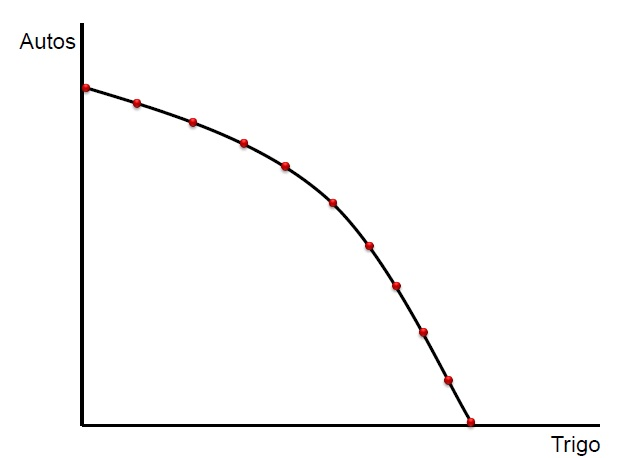
\includegraphics[scale=0.6]{../Tema_11.3_frontera.jpg}
\end{center}
\end{frame}

\begin{frame}
\frametitle{Frontera de posibilidades}
\begin{center}
    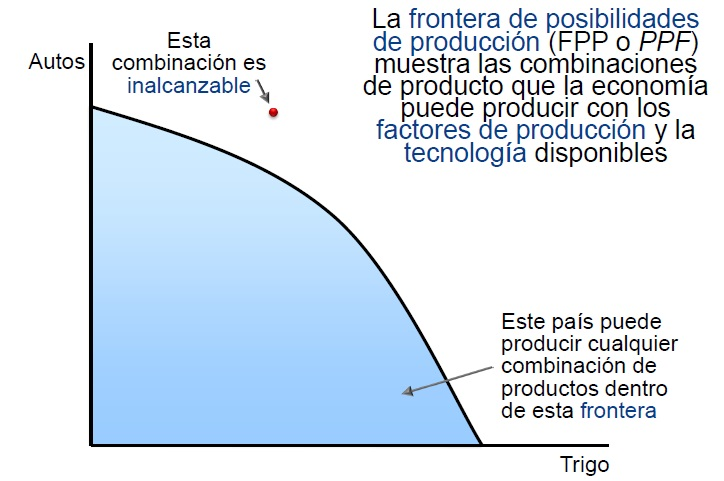
\includegraphics[scale=0.55]{../Tema_11.4_fronteradeposibilidades.jpg}
\end{center}
\end{frame}

\begin{frame}
\frametitle{Fuera de la frontera}
\begin{center}
    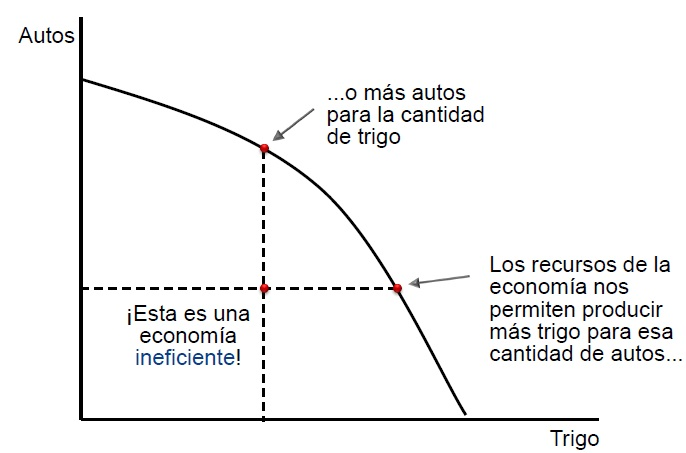
\includegraphics[scale=0.6]{../Tema_11.5_fueradelafrontera.jpg}
\end{center}
\end{frame}

\begin{frame}
\frametitle{Misma frontera}
\begin{center}
    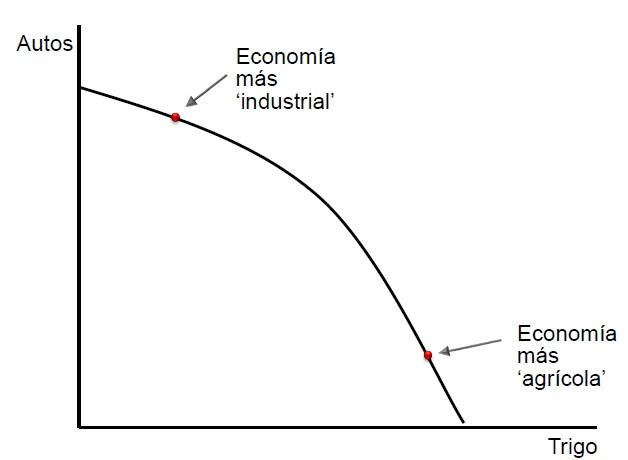
\includegraphics[scale=0.6]{../Tema_11.6_lamismafrontera.jpg}
\end{center}
\end{frame}

\begin{frame}
\frametitle{Cambio en la tecnología}
\begin{center}
    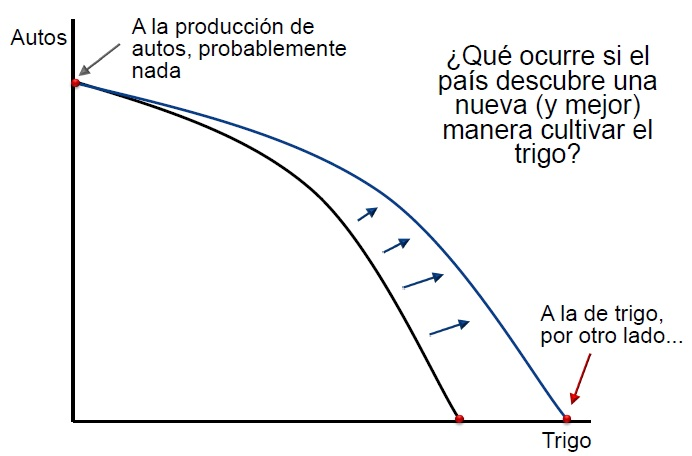
\includegraphics[scale=0.6]{../Tema_11.7_cambiotecnologico.jpg}
\end{center}
\end{frame}

\begin{frame}
\frametitle{Cambio en los factores}
\begin{center}
    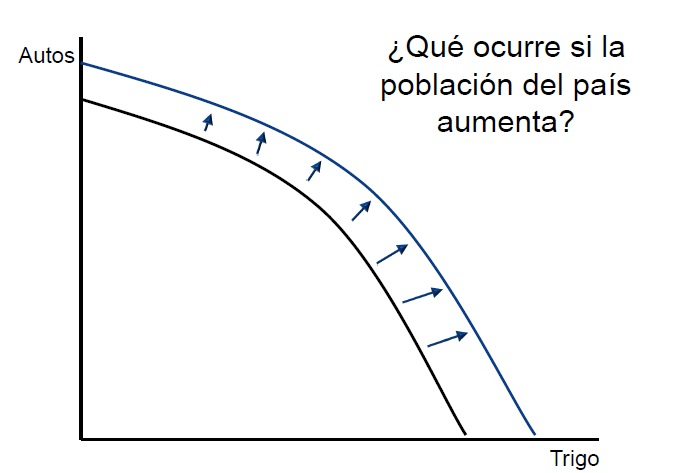
\includegraphics[scale=0.55]{../Tema_11.8_cambioenlosfactores.jpg}
\end{center}
\end{frame}

\begin{frame}
\frametitle{Shock exógeno}
\begin{center}
    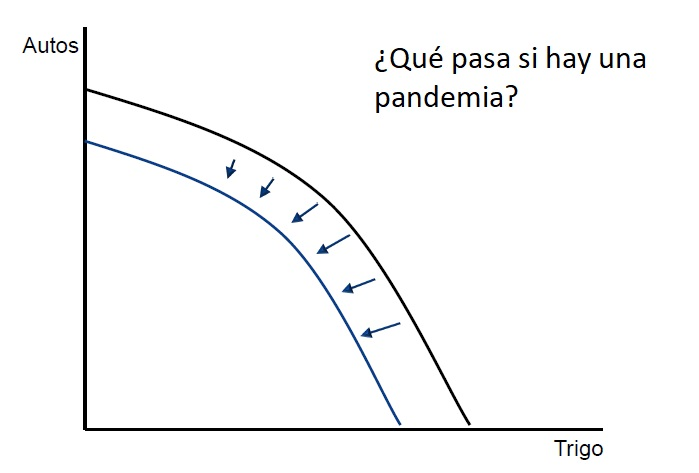
\includegraphics[scale=0.6]{../Tema_11.9_pandemia.jpg}
\end{center}
\end{frame}

\begin{frame}
\frametitle{Cambios en el equilibrio}
\begin{center}
    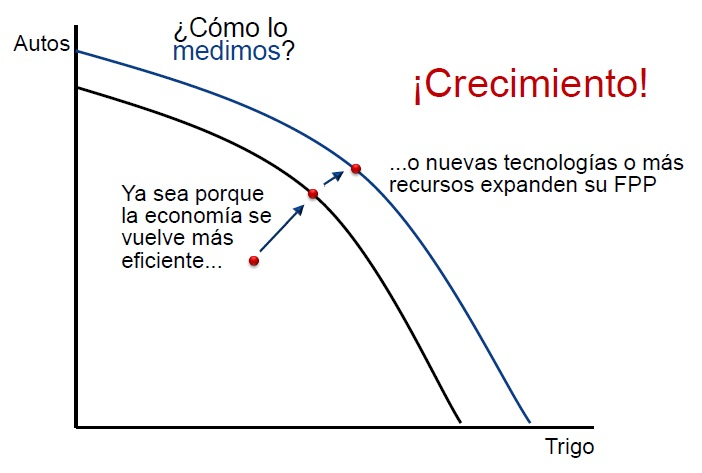
\includegraphics[scale=0.6]{../Tema_11.10_crecimiento.jpg}
\end{center}
\end{frame}

\begin{frame}
\frametitle{Luces nocturnas}
\begin{center}
    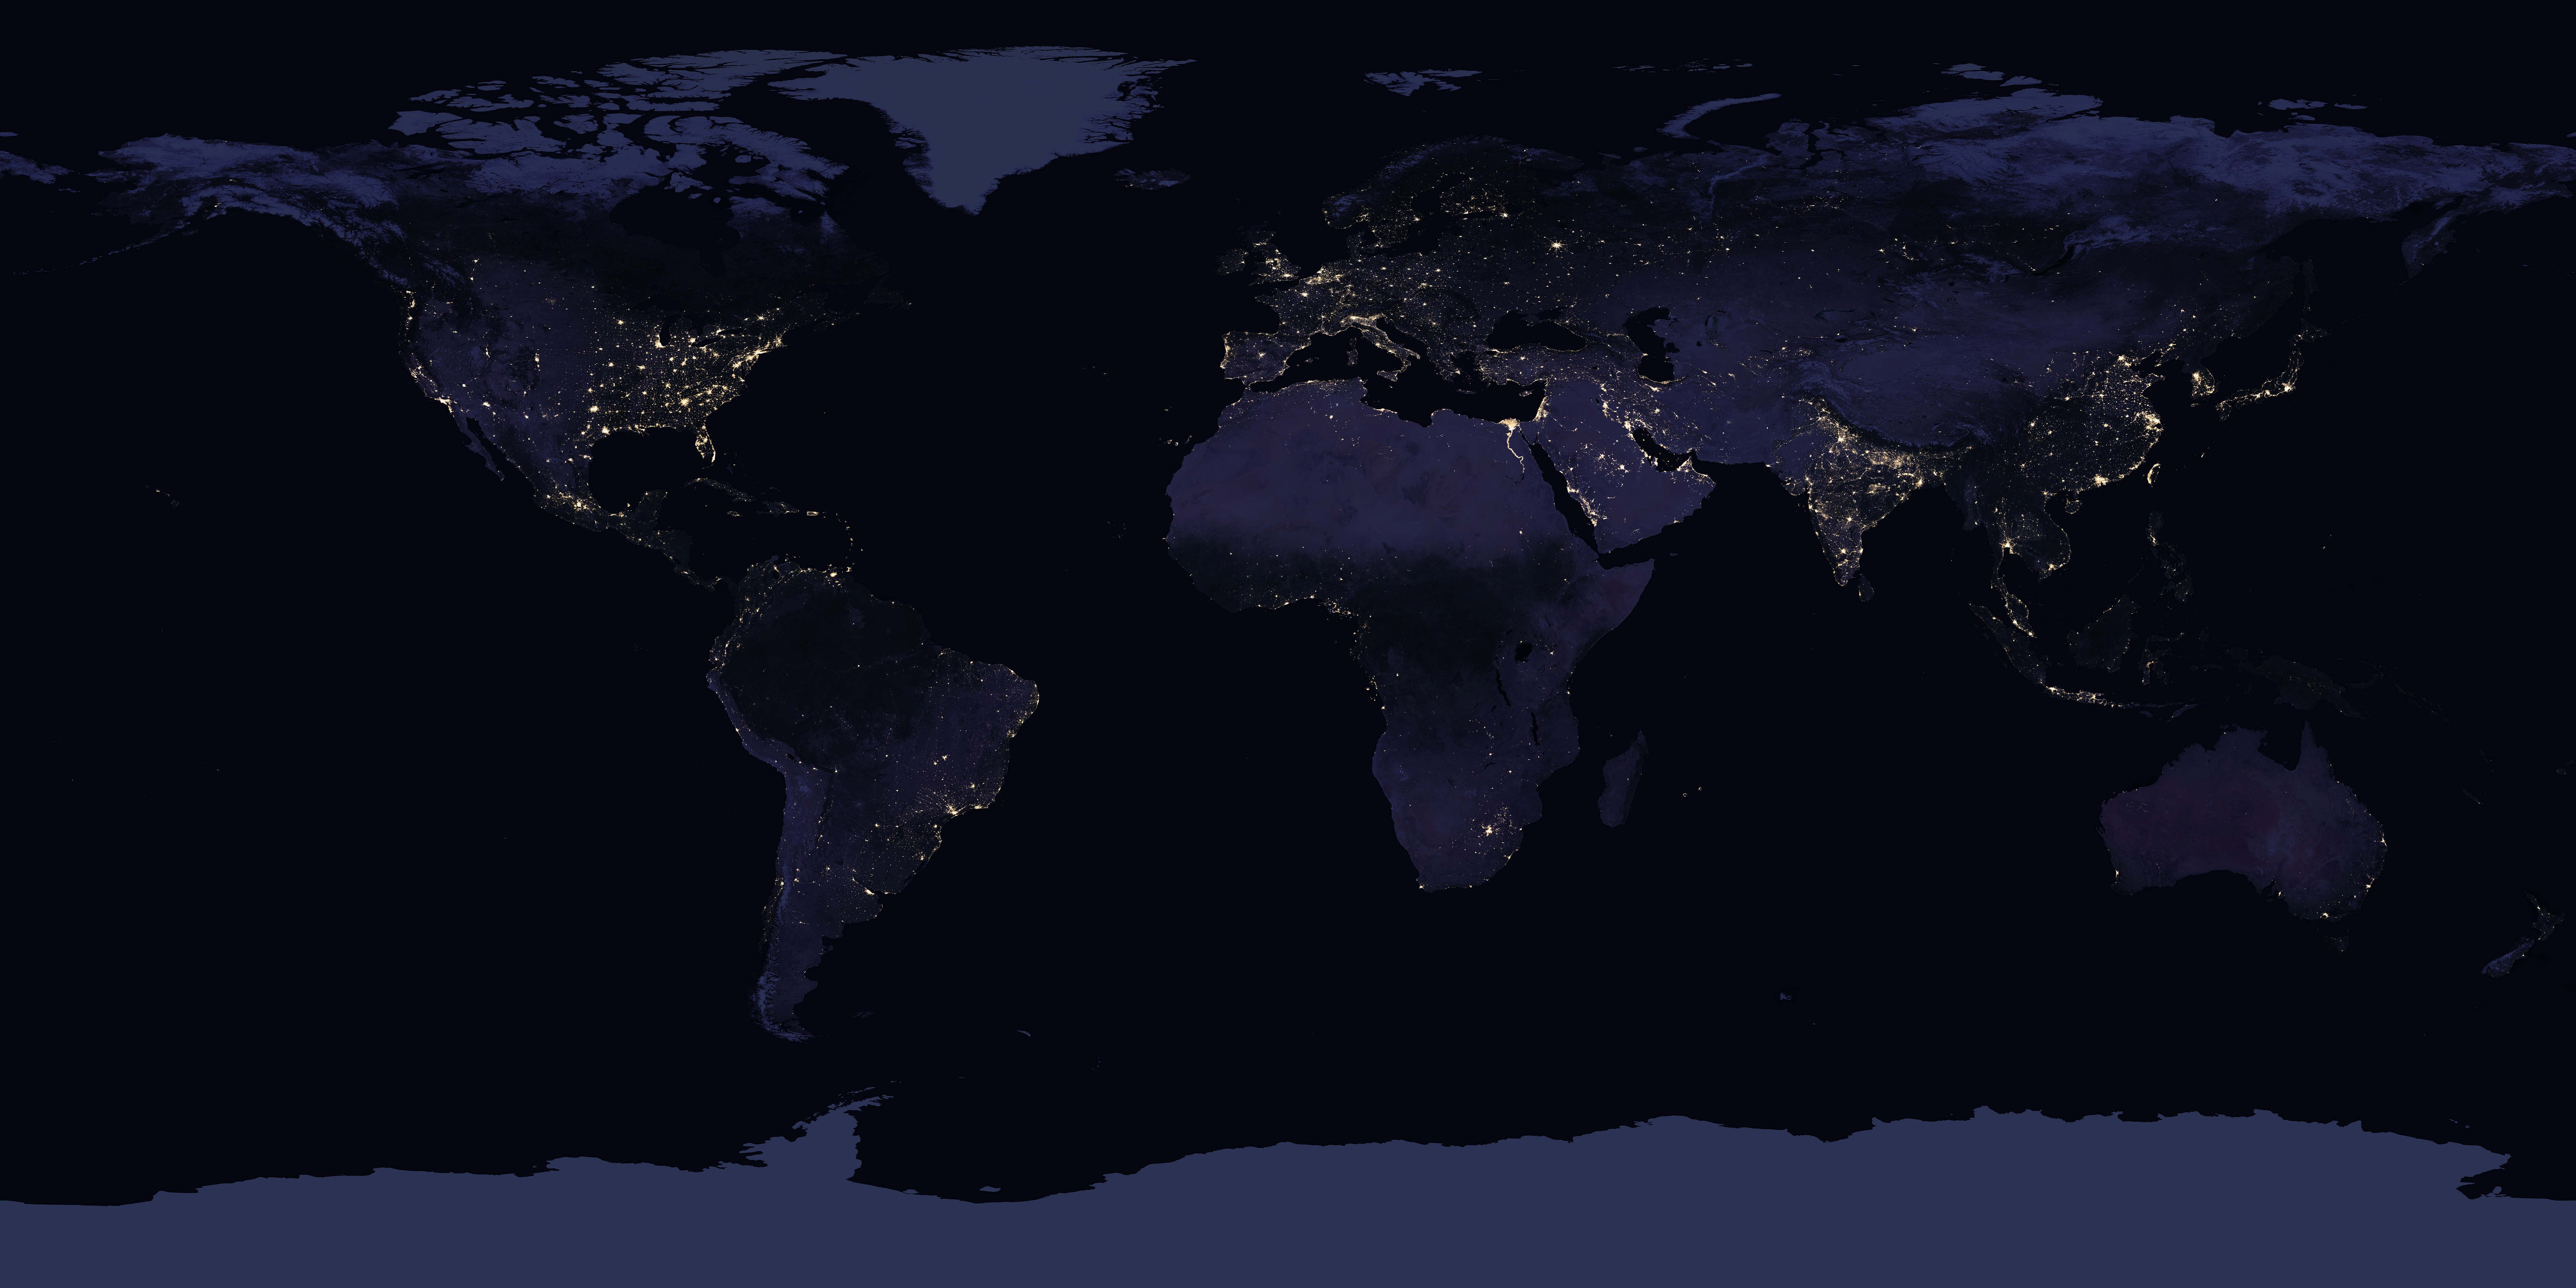
\includegraphics[scale=0.06]{../Tema_11.11_crecimiento2.jpg}
\end{center}
Fuente: \href{https://www.nasa.gov/feature/goddard/2017/new-night-lights-maps-open-up-possible-real-time-applications}{NASA}
\end{frame}

\begin{frame}
\frametitle{Crecimiento}
\begin{center}
    \href{https://ourworldindata.org/grapher/gdp-per-capita-worldbank} {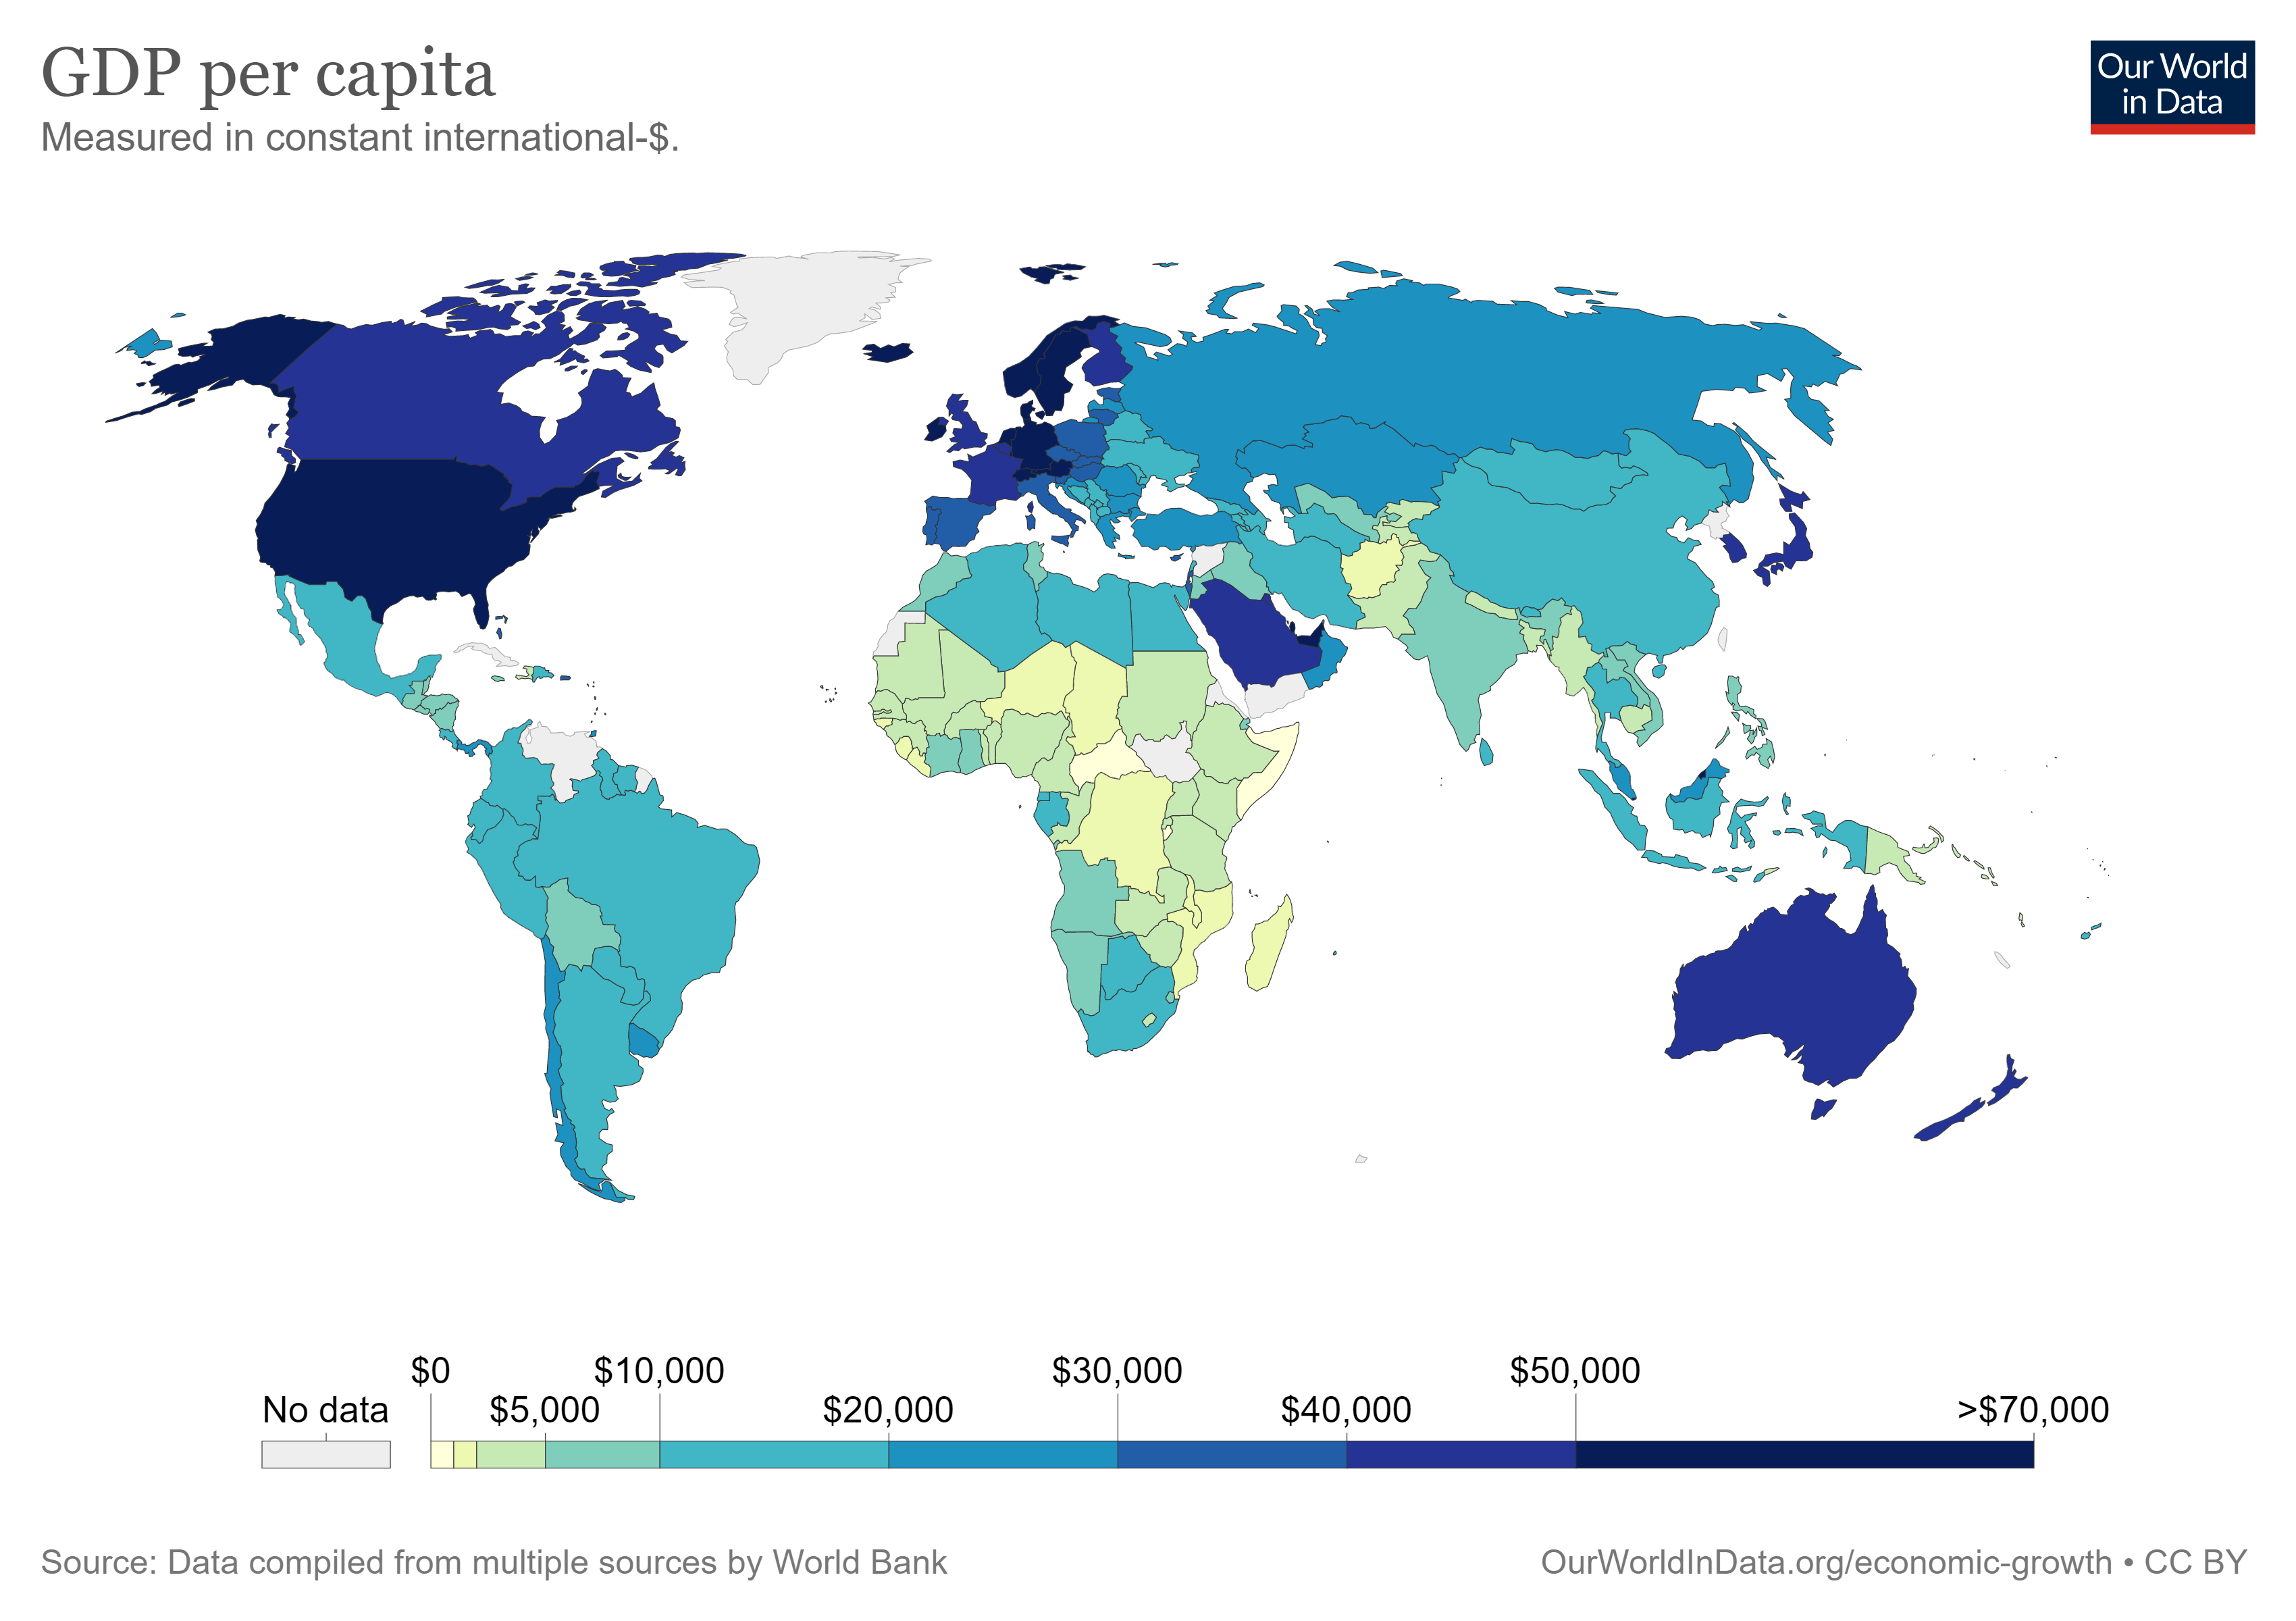
\includegraphics[width=0.8\textwidth]{../Figures/gdppc2020.png}}
\end{center}
Fuente: Our World in Data
\end{frame}

\begin{frame}{Crecimiento del GDP per cápita}
    \begin{figure} [H]   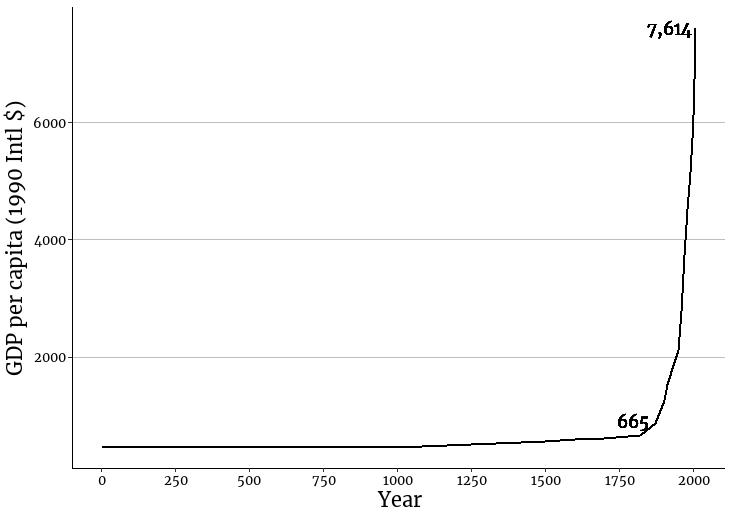
\includegraphics[scale=0.5]{../Figures/C17.1.png}
\end{figure}
\end{frame}

\begin{frame}{¿Qué generó el crecimiento explosivo?}
    \begin{itemize}
    \item \textbf{Revolución industrial (desde mediados del Siglo XVIII)}
    \begin{itemize}
        \item La máquina a vapor generó una potencialidad de expansión en la producción junto con los ferrocarriles y la industria textil produjeron un aumento en el nivel de vida sin precedentes
    \end{itemize}
    
    \item \textbf{Revolución francesa (1789)}
    \begin{itemize}
        \item Permitió la movilidad social
        \item Se pasó de una sociedad estamental a una sociedad libre: mayor libertad para elegir los trabajos y ocupaciones según sus preferencias y capacidades
    \end{itemize}
     \item \textbf{Constitución de EEUU (1787)}
     \begin{itemize}
        \item Fuerte contraste con el poder absolutista de los monarcas europeos
        \item Fuertes restricciones al Estado y lo que éste podía hacer
        \item La emergencia de los gobiernos republicanos con división de poderes implicó un cambio radical en la calidad de la gestión de los recursos públicos
    \end{itemize}
\end{itemize}
\end{frame}

%\begin{frame}{Felicidad y nivel de ingreso}
%    \begin{figure} [H]   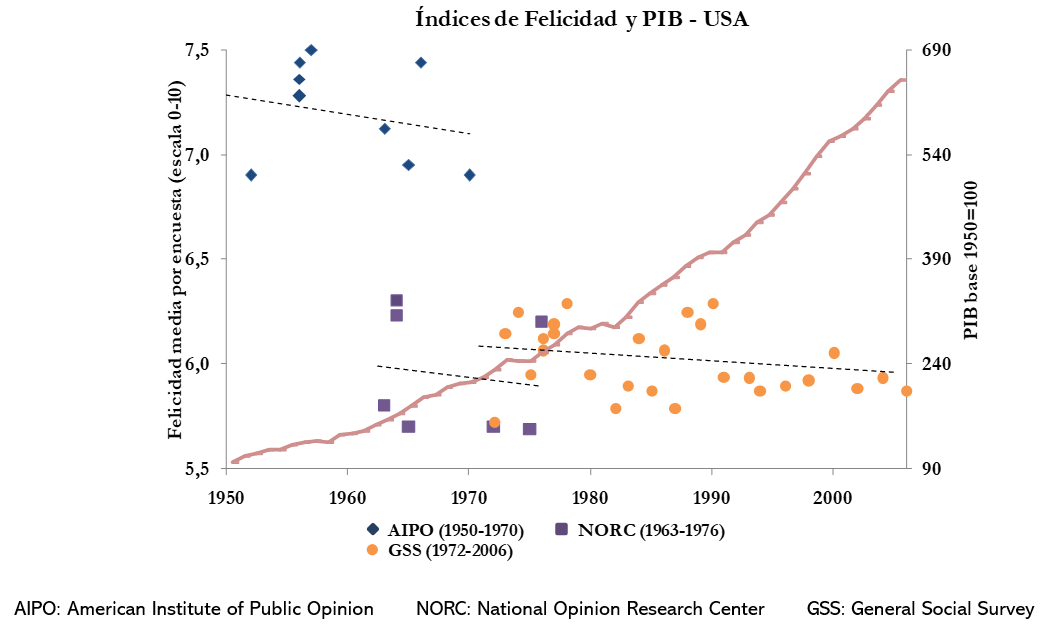
\includegraphics[scale=0.5]{../Figures/C17.2.png}
%\end{figure}
%\end{frame}

%\begin{frame}
%\frametitle{Idea más amplia de bienestar}
%\begin{itemize}
%    \item Enfoque de capacidades de Amartya Sen
%    \begin{itemize}
%        \item No es lo que una persona tiene, sino lo que ella es y puede hacer \\
%        - Capacidades para alcanzar su potencial como ser humano
%        \item ¿Disparidad entre los ingresos y las ventajas reales? \\
%        - Heterogeneidades personales, diversidad ambiental, diferencias en el clima social, distribución de recursos dentro de la familia, etc.
%    \end{itemize}
%    \item Índice de Desarrollo Humano (HDI) del PNUD
%    \begin{itemize}
%        \item Ingresos (PBI per cápita ajustado por PPP)
%        \item Longevidad (esperanza de vida al nacer)
%        \item Conocimiento (alfabetización y años de estudio0
%    \end{itemize}
%    \end{itemize}
%\end{frame}

%\begin{frame}
%\frametitle{HDI (2017)}
%\begin{center}
%    \href{https://ourworldindata.org/grapher/human-development-index?country=~ZWE} {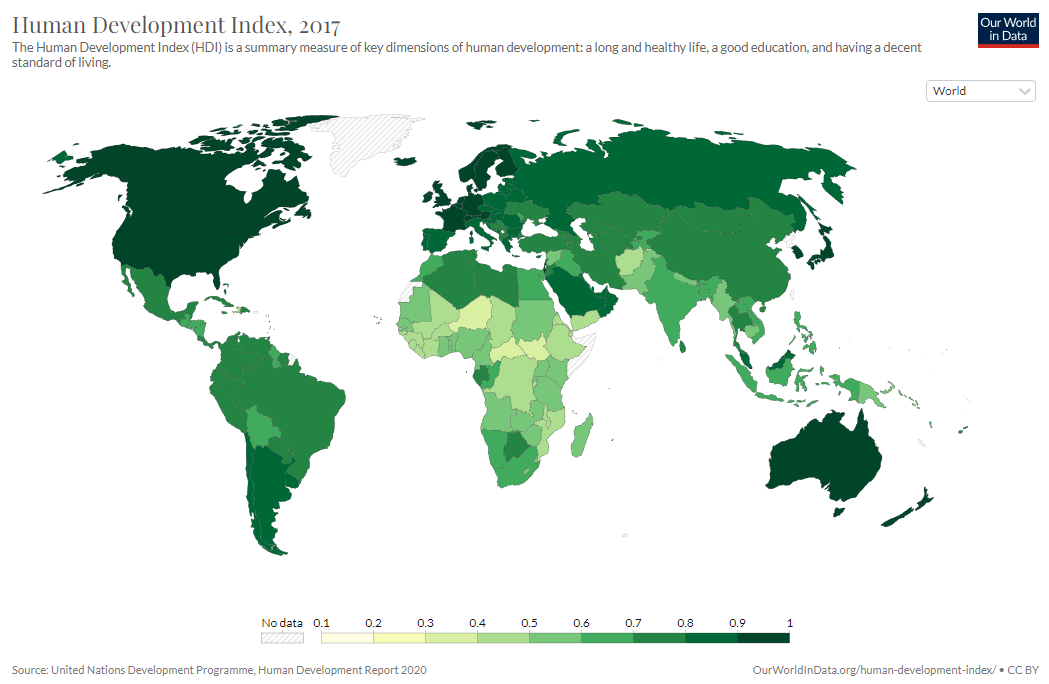
\includegraphics[scale=0.35]{../Figures/Tema_11.27_hdi_PBI.png}}
%\end{center}
%Fuente: Our World in Data
%\end{frame}

\begin{frame}
\frametitle{PBI y desarrollo}
\begin{center}
    \href{https://ourworldindata.org/grapher/hdi-vs-gdp-per-capita} {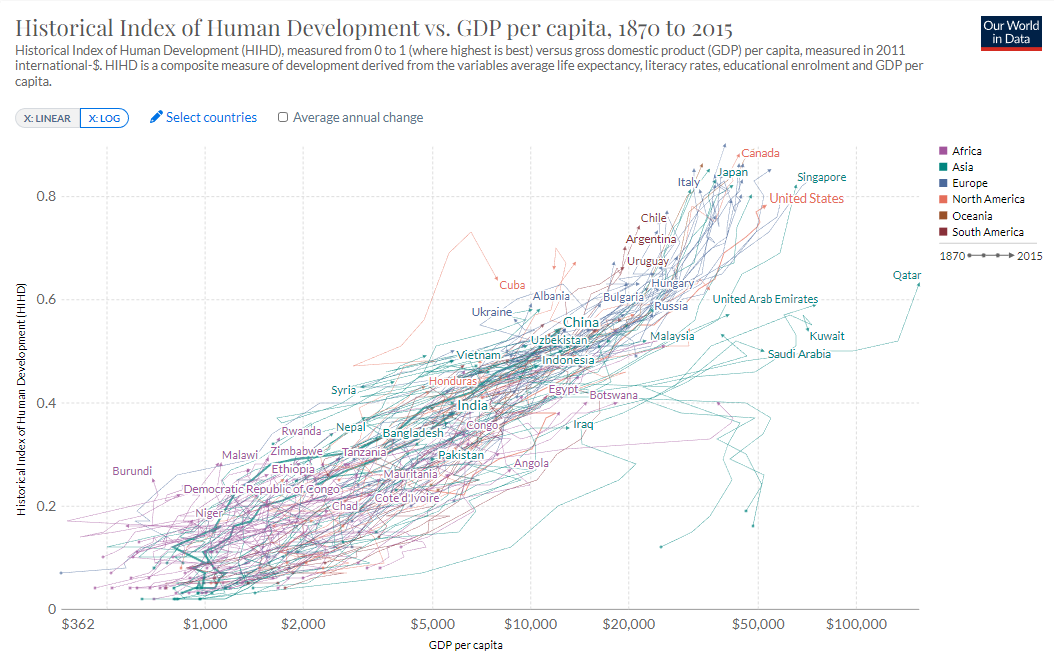
\includegraphics[scale=0.35]{../Tema_11.27_hdi_2.png}}
\end{center}
Fuente: Our World in Data
\end{frame}

\begin{frame}{Fuentes del crecimiento}
   \begin{equation}
    Y = AF(K,L,H,RN),
\end{equation} 
\begin{itemize}
    \item El crecimiento viene de la acumulacion de factores o de la tecnologia?
    \item El hallazgo de Solow
    \item Hong Kong vs Singapur
\end{itemize}
\end{frame}

\begin{frame}{Un ejemplo de productividad}
    \begin{figure} [H]   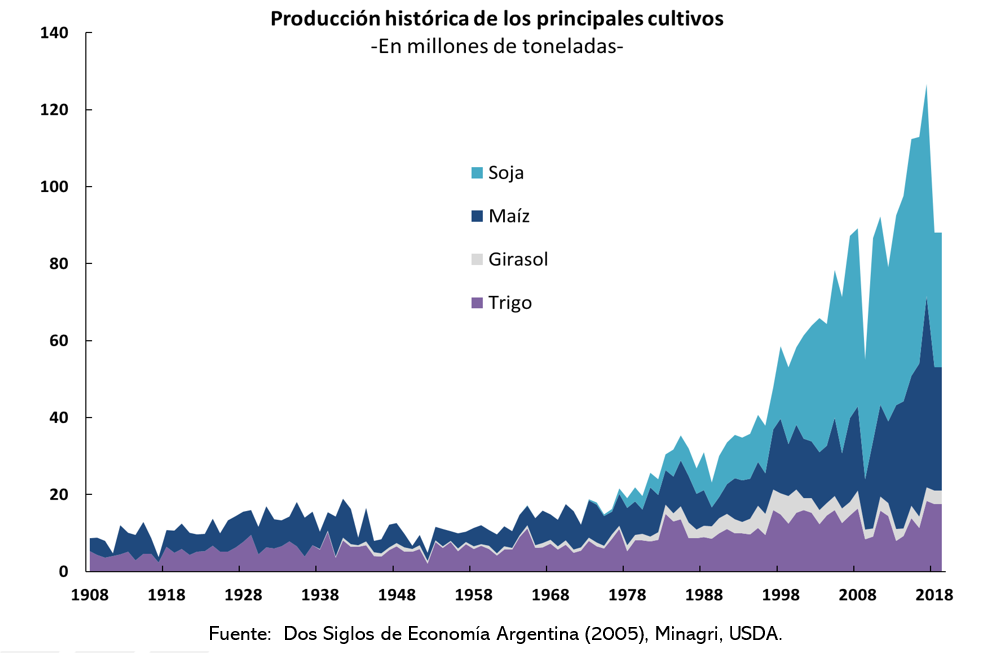
\includegraphics[scale=0.55]{../Figures/C17.3.png}
\label{fig:17.3}
\end{figure}
\end{frame}


\begin{frame}{La descomposición de crecimiento para Argentina}
    \begin{figure} [H]   
        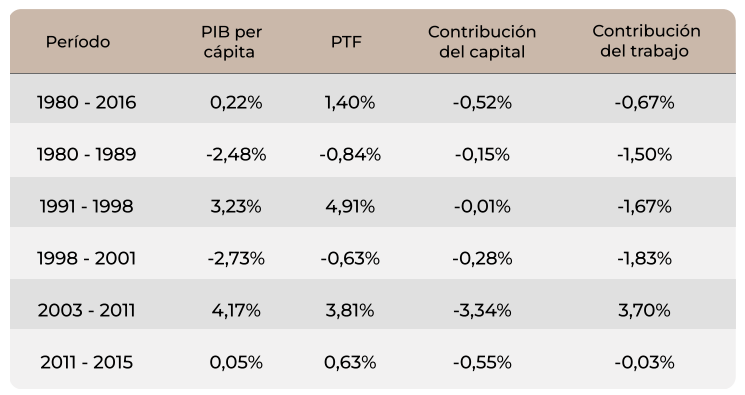
\includegraphics[scale=0.55]{../Figures/C30.8.png}
        \caption{\textbf{Descomposición del crecimiento de Argentina}}
    \end{figure}
\end{frame}

\begin{frame}{Instituciones y Crecimiento}
    \begin{itemize}
        \item Dijimos que las instituciones son las reglas del juego en una sociedad
        \item \textbf{Instituciones económicas e instituciones políticas}
        \item Afectan de manera directa a los incentivos
        \item Establecen los incentivos para la innovación y el desarrollo tecnológico
        \item ¿Podemos evaluar de manera empírica el rol de las instituciones?
    \end{itemize}
    
    \begin{figure}[H]
        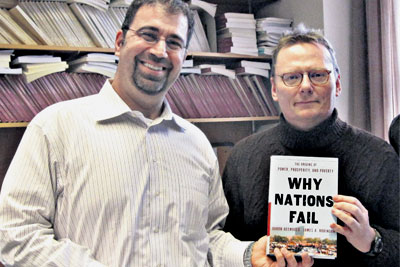
\includegraphics[scale=0.5]{../Figures/Acemoglurobinson.png}
    \end{figure}
\end{frame}

\begin{frame}{Instituciones}
    
    \begin{figure}[H]
        \begin{center}
            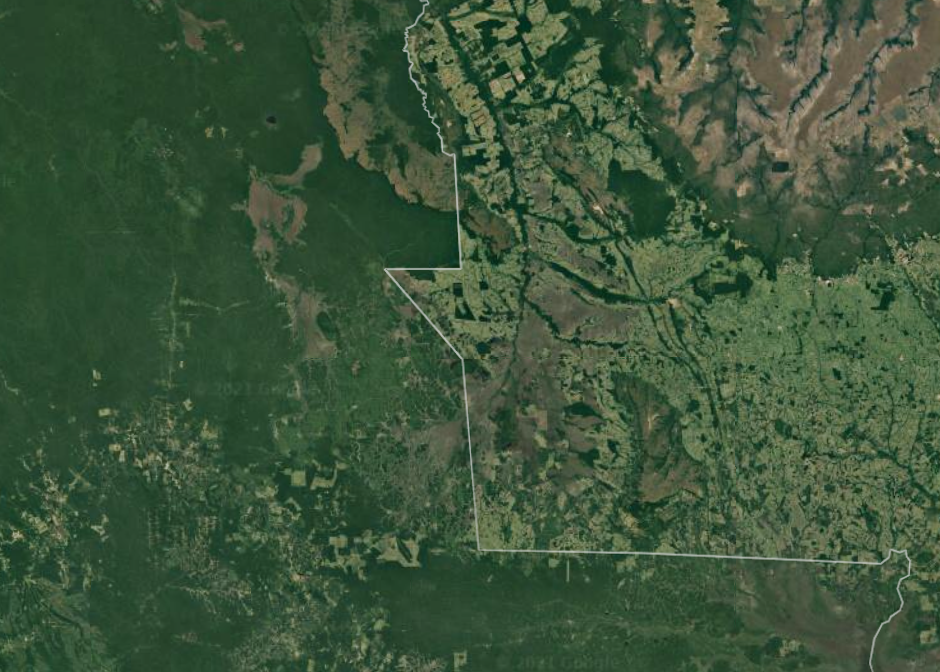
\includegraphics[width=0.8\textwidth]{../Figures/C26.2.png}
        \end{center}
        \caption{\textbf{Frontera entre Bolivia (izquierda) y Brazil}}
    \end{figure}
\end{frame}


\begin{frame}{Instituciones}
    \begin{figure}[H]
    \begin{center}
    \includegraphics[width=0.8\textwidth]{../Figures/C26.3.png}
    \end{center}
    \caption{\textbf{Península de Corea de noche}}
    \label{fig:korea}
    \end{figure}
\end{frame}

\begin{frame} 
\frametitle{Desigualdad del Ingreso}
\begin{itemize}
\item Hay dos criterios para evaluar una asignación específica: 
\begin{itemize}
    \item Eficiencia
    \item Equidad
\end{itemize}
\item ¿Existe un trade off entre eficiencia y equidad? No debería...
\end{itemize}
\end{frame}


\begin{frame} 
\frametitle{Desigualdad del Ingreso}
\begin{itemize}
\item Hay algunos factores importantes que determinan si una asignación es muy desigual: \begin{itemize}
    \item Diferencias en el poder de negociación
    \item Diferencias en sus dotaciones
    \item Instituciones
\end{itemize}
\item Para evaluar la desigualdad, los economistas a menudo usan unas medidas llamadas Coeficiente de Gini y Curva de Lorenz
\end{itemize}
\end{frame}

\begin{frame} 
\frametitle{El Coeficiente de Gini}
\begin{itemize}
\item El coeficiente de Gini se basa en las diferencias en los ingresos, la riqueza o alguna otra medida entre las personas
\item El coeficiente de Gini tiene la ventaja de que incluye información sobre todos, no solo los ricos y los pobres, sino también aquellos ``en el medio''
\item Se calcula a partir de dos datos:
        \begin{itemize}
            \item El promedio de las diferencias entre las personas
            \item El ingreso promedio de las personas
        \end{itemize}
\end{itemize}
\end{frame}

\begin{frame} 
\frametitle{El Coeficiente de Gini}
\begin{itemize}
\item Coeficiente Gini = $0,5$ x  $\frac{\text{Diferencia Promedio}}{\text{Ingreso Promedio}}$
\item En la práctica, cuando calculamos el coeficiente de Gini, obtenemos un número entre 0 (igualdad perfecta) y 1 (desigualdad extrema). 
\item Cuanto más desigualmente se distribuyen los recursos entre los miembros de la población, mayor es el coeficiente de Gini.
\end{itemize}
\end{frame}


\begin{frame} 
\frametitle{Un ejemplo}
\begin{itemize}
    \item Los círculos son personas y los números dentro de los círculos son los ingresos recibidos
    \item Los números al lado de las flechas son las diferencias entre las dos personas, indicadas por las flechas
\end{itemize} 
    \begin{center}    
    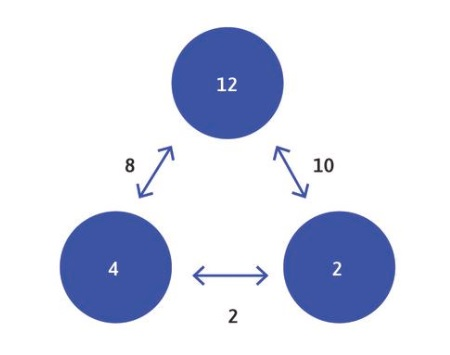
\includegraphics[scale=0.5]{../Tema_04.15_gini.jpg}
    \end{center}
\end{frame}

\begin{frame} 
\frametitle{Un ejemplo}
\begin{itemize}
    \item El promedio de las diferencias entre las personas es \\ (10 + 8 + 2) / 3 = 20/3 = 6,67 \\ \vspace{3mm}
    \item El ingreso promedio de las personas es \\ (12 + 4 + 2) / 3 = 6
\end{itemize}
\vspace{3mm}

El coeficiente de Gini es igual a 
\begin{center}
    0,5 $ \frac{6,67}{6} = 0,56$
\end{center}
\end{frame}

\begin{frame} 
\frametitle{La curva de Lorenz}
\begin{itemize}
\item Es una herramienta útil para observar la distribución completa del ingreso o la riqueza que representa y comparar las distribuciones del ingreso o la riqueza entre los países
\item Es una representación gráfica de la desigualdad de cierta cantidad, como la riqueza o el ingreso
\item Indica cuánta disparidad hay en el ingreso, o en cualquier otra medida, a través de la población
\end{itemize}
\end{frame}

\begin{frame} 
\frametitle{La curva de Lorenz}
\begin{itemize}
\item Los individuos se organizan en orden ascendente según el ingreso que tienen, y la parte acumulada del ingreso se grafica contra la parte acumulada de la población
\item Para la igualdad completa de ingresos, la curva de Lorenz sería una línea recta con una pendiente igual a uno
\item La medida en que la curva cae por debajo de esta línea de igualdad perfecta es una medida de la desigualdad
\end{itemize}
\end{frame}

\begin{frame} 
\frametitle{Curva de Lorenz}
\begin{figure} [H]
\centering
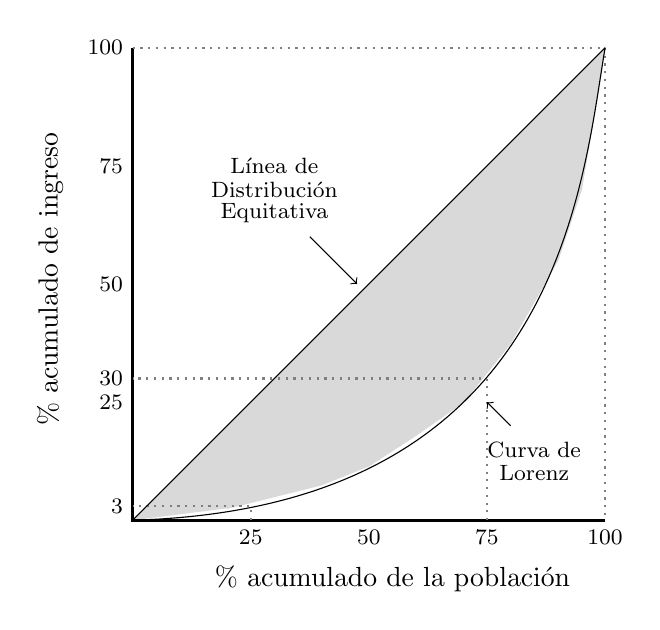
\begin{tikzpicture}[scale=0.6]
\draw[fill,gray!30] (0,0)--(10,10)--(9.5,7)--(9,5.5)--(8,3.75)--(7,2.5)--(6,1.8)--(5,1.15)--(4,0.75)--(2,0.25);
\draw[very thick,-] (0,10) node[above]{}--(0,0)--(10,0) node[right]{};
\draw[thick, dotted, gray] (0,10)--(10,10)--(10,0);
\draw[thick, dotted, gray] (2.5,0)--(2.5,0.3)--(0,0.3);
\draw[thick, dotted, gray] (7.5,0)--(7.5,3)--(0,3);
\draw[thin] (0,0)--(10,10);
\draw[thin] (0,0)..controls (9,0.25) and (9.5,7)..(10,10);
\node at (-1.75, 5){\rotatebox{90}{ \% acumulado de ingreso}};
\node[] at (5.5,-1.25) { \% acumulado de la población};
\node[below] at (2.5,0){\footnotesize 25};
\node[below] at (5,0){\footnotesize 50};
\node[below] at (7.5,0){\footnotesize 75};
\node[below] at (10,0){\footnotesize 100};
\node[left] at (0,0.3){\footnotesize 3};
\node[left] at (0,2.5){\footnotesize 25};
\node[left] at (0,3){\footnotesize 30};
\node[left] at (0,5){\footnotesize 50};
\node[left] at (0,7.5){\footnotesize 75};
\node[left] at (0,10){\footnotesize 100};
\node[] at (3,7.5) {\footnotesize Línea de };
\node[] at (3,7) {\footnotesize Distribución};
\node[] at (3,6.5) {\footnotesize Equitativa };
\draw[thin, ->] (3.75,6)--(4.75,5);
\node[] at (8.5,1.5) {\footnotesize Curva de };
\node[] at (8.5,1) {\footnotesize Lorenz };
\draw[thin, ->] (8,2)--(7.5,2.5);
\end{tikzpicture}
\end{figure} 
\end{frame}

\begin{frame} 
\frametitle{Un ejemplo aplicado}
    \begin{center}    
    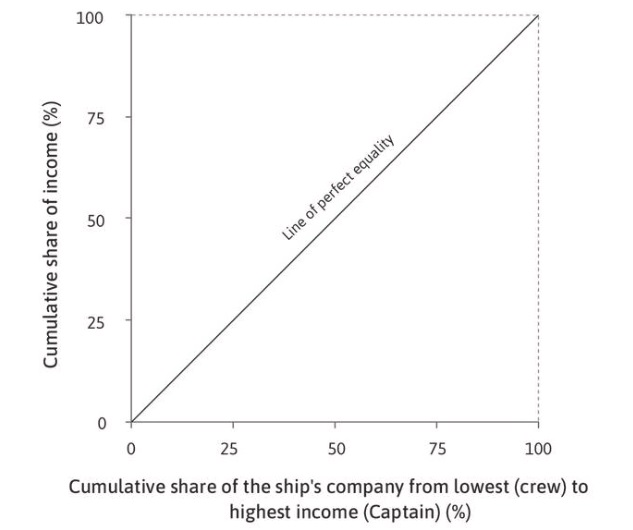
\includegraphics[scale=0.55]{../Tema_04.16_lorenz1.jpg}
    \end{center}
\end{frame}

\begin{frame} 
\frametitle{Un ejemplo aplicado}
    \begin{center}    
    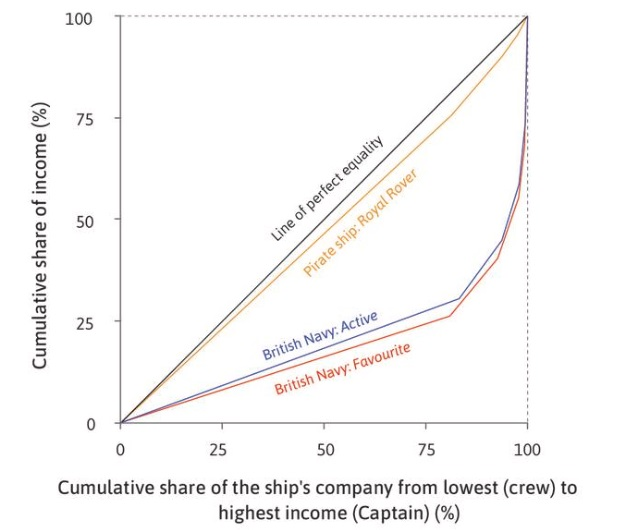
\includegraphics[scale=0.55]{../Tema_04.17_lorenz2.jpg}
    \end{center}
\end{frame}

\begin{frame} 
\frametitle{El coeficiente de Gini y la curva de Lorenz}
\begin{itemize}
\item Si todos tienen el mismo ingreso (no hay desigualdad de ingresos), el coeficiente de Gini toma un valor de 0. 
\begin{itemize}
    \item Esto se debe a que la curva de Lorenz sería exactamente la línea de la igualdad perfecta, por lo que no habría área entre los dos
\end{itemize}
\item $G=\frac{A}{A+B}$
\item Este método de cálculo del Gini solo da una aproximación. La aproximación del área sólo es precisa cuando la población es grande
\end{itemize}
\end{frame}

\begin{frame} 
\frametitle{Un ejemplo aplicado}
    \begin{center}    
    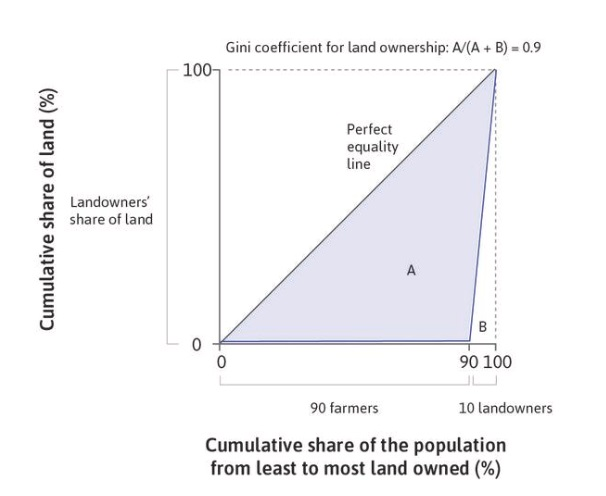
\includegraphics[scale=0.55]{../Tema_04.18_lorenz3.jpg}
    \end{center}
\end{frame}

\begin{frame} 
\frametitle{Un ejemplo aplicado}
    \begin{center}    
    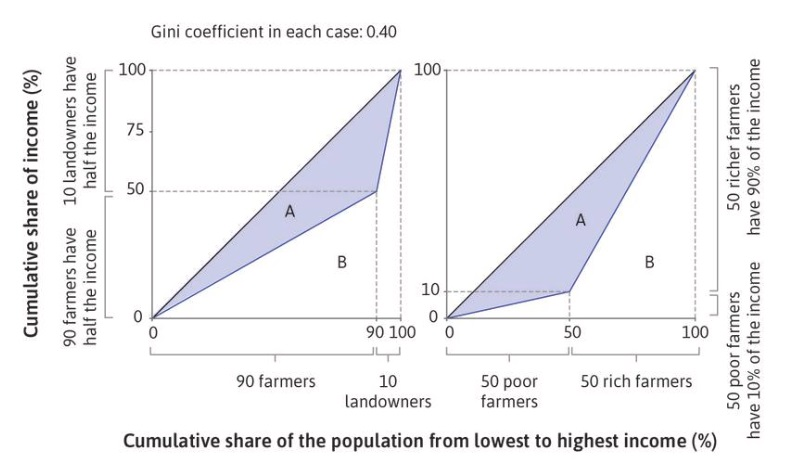
\includegraphics[scale=0.55]{../Tema_04.20_variedaddesigual.jpg}
    \end{center}
\end{frame}

\begin{frame} 
\frametitle{Diferentes variedad de desigualdad}
\begin{itemize}
\item En la figura anterior hay dos sociedades con el mismo coeficiente de Gini.
\item El área $\frac{A}{A + B}$ es la misma en cada curva de Lorenz, pero la distribución del ingreso está lejos de ser idéntica.
\item En la sociedad de la izquierda, la mitad del ingreso total se divide entre 90 agricultores mientras que 10 terratenientes obtienen la mitad restante. 
\item En la sociedad que se muestra a la derecha, 50 agricultores pobres obtienen una décima parte de los ingresos para dividirse entre ellos y 50 agricultores más ricos dividen el 90\% restante.
\end{itemize}
\end{frame}

\begin{frame} 
\frametitle{Diferentes variedad de desigualdad}
\begin{itemize}
\item ¡No todas las desigualdades son iguales!
\item No es lo mismo que una sociedad sea altamente desigual porque hay un pequeño número de personas excepcionalmente ricas y todos los demás están en una situación de buena posición económica o que sea desigual porque hay un pequeño número de personas muy pobres, y todos los demás están en mejores condiciones
\item Estas dos sociedades podrían tener el mismo coeficiente de Gini, pero pensaríamos que son bastante diferentes en la naturaleza de la desigualdad que experimentan
\end{itemize}
\end{frame}

\begin{frame} 
\frametitle{Gini Argentina}

\end{frame}

\end{document}